\section{Hodge Index Theorem by Linear Algebra}

\subsection{Linear algebra}

    \begin{proposition}\label{prop:of_type_1_n-1_if_x2_positive_has_two_components}
        Let \(V\) be a real vector space of dimension \(n\) with a non-degenerated symmetric bilinear form \(\langle-,-\rangle\).
        Consider the subset
        \[ S = \{x \in V \mid \langle x, x \rangle > 0\}. \]
        Suppose that \(S\neq \emptyset\) and there exists \(z \in V\) such that \(z^\perp \cap S = \emptyset\), then the signature of \(\langle-,-\rangle\) is of type \((1, n-1)\), where \(z^\perp = \{v \in V \mid \langle z, v \rangle = 0\}\).
    \end{proposition}
    \begin{proof}
        Choose \(h \in S\).
        We claim that the restriction of \(\langle-,-\rangle\) on \(h^\perp\) is negative definite.
        First, the restriction is non-degenerated.
        Otherwise, note that \(h\) and \(h^\perp\) generate \(V\). 
        If there exists \(0 \neq x \in h^\perp\) such that \(\langle x, y \rangle = 0\) for all \(y \in h^\perp\), then in particular \(\langle x, h \rangle = 0\), 
        thus \(x \in h^\perp\) and \(x \in V^\perp = \{0\}\), which is a contradiction.
        
        Hence if the restriction is not negative definite, then there exists \(x \in h^\perp\) such that \(\langle x, x \rangle > 0\).
        Then consider the subspace \(V_0\) generated by \(h\) and \(x\).
        We have \(h^2,x^2 > 0\) and \(h \cdot x = 0\), thus the restriction of \(\langle-,-\rangle\) on \(V_0\) is of type \((2, 0)\).
        Hence \(z^\perp \cap V_0 = \{0\}\).
        However, consider the dimension count
        \[ \dim(z^\perp + V_0) = \dim(z^\perp) + \dim(V_0) - \dim(z^\perp \cap V_0) = (n-1) + 2 - 0 = n + 1 > n = \dim(V), \]
        which is a contradiction.
    \end{proof}

    \begin{remark}\label{rmk:of_type_1_n-1_iff_x2_positive_has_two_components}
        Geometrically, we have the following equivalent statement: 
        \begin{enumerate}
            \item \(S \neq \emptyset\) and there exists \(z \in V\) such that \(z^\perp \cap S = \emptyset\);
            \item the signature of \(\langle-,-\rangle\) is of type \((1, n-1)\);
            \item the set \(S\) has two connected components.
        \end{enumerate}

        We have shown \((a) \Rightarrow (b)\) in \cref{prop:of_type_1_n-1_if_x2_positive_has_two_components}.
        If the signature of \(\langle-,-\rangle\) is of type \((1, n-1)\), then we can choose a basis such that the matrix of \(\langle-,-\rangle\) is
        \[ \begin{pmatrix}
            1 & 0 & 0 & \cdots & 0 \\
            0 & -1 & 0 & \cdots & 0 \\
            0 & 0 & -1 & \cdots & 0 \\
            \vdots & \vdots & \vdots & \ddots & \vdots \\
            0 & 0 & 0 & \cdots & -1
        \end{pmatrix}. \]
        Then the set \(S\) is given by the equation
        \[ x_1^2 - x_2^2 - \cdots - x_n^2 > 0, \]
        which has two connected components, thus \((b) \Rightarrow (c)\).
        Finally, if \(S\) has two connected components, then for any \(z \in S\), we claim that \(z^\perp \cap S = \emptyset\).
        Otherwise, there exists \(x \in z^\perp \cap S\).
        Considering on the subspace \(V_0\) generated by \(z\) and \(x\), we see that \(z\) and \(-z\) lie in the same connected component of \(S\).
        For every \(y \in S\), assume \(z.y > 0\) (otherwise replace \(z\) by \(-z\)), then the line segment \(tz + (1-t)y\) for \(t \in [0,1]\) connects \(z\) and \(y\) in \(S\).
        Hence \(S\) is path connected, which is a contradiction.
    \end{remark}

    \begin{example}\label{rmk:space_time_like}
        Let \(V = \bbR^4 = \{(t,x,y,z) \mid t,x,y,z \in \bbR\}\) be the Minkowski space with the bilinear form
        \[ \langle (t,x,y,z), (t',x',y',z') \rangle = tt' - xx' - yy' - zz'. \]
        Then (the closure of) the set \(S = \{(t,x,y,z) \in V \mid t^2 - x^2 - y^2 - z^2 > 0\}\) is called the set of \emph{light cone}.
        It has two connected components, which are called the \emph{future light cone} and the \emph{past light cone}; see \cref{fig:light_cone}.
    \end{example}
    \begin{figure}[!h]
        \centering
        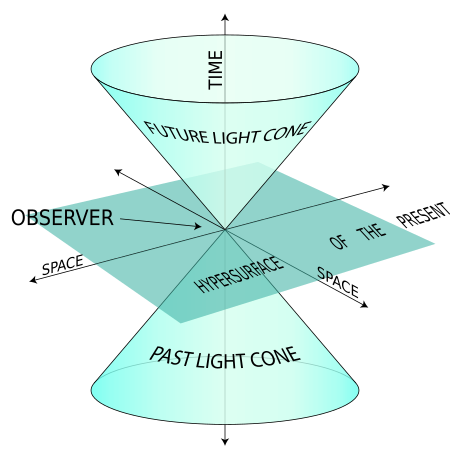
\includegraphics[width=0.3\textwidth]{World_line.svg.png}
        \caption{Light cone in Minkowski space, from \url{https://en.wikipedia.org/wiki/Light_cone}}
        \label{fig:light_cone}
    \end{figure}


\subsection{Hodge index theorem for surfaces}

    \begin{lemma}[Riemann-Roch theorem for surfaces]\label{lem:Riemann_Roch_for_surfaces}
        Let \(X\) be a smooth projective surface over an algebraically closed field \(\kkk\) and \(D\) a divisor on \(X\).
        Then we have
        \[ h^0(\calO_X(D)) - h^1(\calO_X(D)) + h^0(\calO_X(K_X-D)) = \chi(\calO_X) + \frac{1}{2}D \cdot (D - K_X), \]
        where \(K_X\) is the canonical divisor of \(X\).
    \end{lemma}

    \begin{lemma}\label{lem:intersection_of_curve_on_surface}
        Let \(X\) be a smooth projective surface over an algebraically closed field \(\kkk\) and \(D\) a divisor on \(X\).
        If \(D^2 > 0\), then at least one of \(D\) and \(-D\) is pseudo-effective.
    \end{lemma}
    \begin{proof}
        Suppose for contradiction that both \(D\) and \(-D\) are not pseudo-effective.
        In particular, we have \(h^0(\calO_X(mD)) = 0\) for all \(m > 0\).
        By \cref{lem:Riemann_Roch_for_surfaces}, we have
        \[ h^0(\calO_X(K_X - mD)) \geq \chi(\calO_X) + \frac{1}{2}mD \cdot (mD + K_X) > 0 \text{ for all } m \gg 0. \]
        Hence there exist effective divisors \(E_m \sim K_X - mD\) for all \(m \gg 0\).
        We have \(-D \sim_\bbQ \frac{1}{m}(E_m - K_X)\) is pseudo-effective, which is a contradiction.
    \end{proof}

    \begin{theorem}\label{thm:Hodge_index_theorem_for_surfaces}
        Let \(X\) be a smooth projective surface over an algebraically closed field \(\kkk\).
        Then the intersection form on \(\NS(X)_\bbR = \NS(X) \otimes_\bbZ \bbR\) is of type \((1, \rho(X)-1)\), where \(\rho(X) = \dim_\bbR \NS(X)_\bbR\) is the Picard number of \(X\).
    \end{theorem}
    \begin{proof}
        Note that both \(\Psef(X) \setminus \{0\}\) and \(-\Psef(X) \setminus \{0\}\) are convex cones in \(\NS(X)_\bbR\) and they are disjoint.
        Hence there exists a hyperplane \(H\) in \(\NS(X)_\bbR\) such that \(H \cap \Psef(X) = \{0\}\) by the geometric form of Hahn-Banach theorem.
        By \cref{lem:intersection_of_curve_on_surface}, 
        \[ H \cap \{D \in \NS(X)_\bbR \mid D^2 > 0\} = \emptyset. \]
        Then the conclusion follows from \cref{prop:of_type_1_n-1_if_x2_positive_has_two_components}.
    \end{proof}

\subsection{Siu's inequality in the surface case}

    \begin{theorem}[Siu's inequality]\label{thm:Siu_inequality}
        Let \(X\) be a smooth projective variety of dimension \(n\) over an algebraically closed field \(\kkk\).
        Let \(A, B\) be nef divisors on \(X\) such that \(A^n > 0\).
        Then we have
        \[ A^n \cdot B^n \leq n (A^{n-1} \cdot B)\cdot (B^{n-1} \cdot A). \]
    \end{theorem}

    In the surface case, it is easy.
    The following is a proof using \cref{thm:Hodge_index_theorem_for_surfaces} and linear algebra.

    \begin{proposition}\label{prop:Siu_inequality_surface_case}
        Let \(V\) be a real vector space of dimension \(n\) with a non-degenerated symmetric bilinear form \(\langle-,-\rangle\) of type \((1, n-1)\).
        Let \(v \in V\) with \(\langle v,v \rangle > 0\).
        Then for any \(w \in V\), we have
        \[ \langle v,v \rangle \cdot \langle w,w \rangle \leq \langle v,w \rangle^2, \]
        and the equality holds if and only if \(v\) and \(w\) are linearly dependent.
    \end{proposition}
    \begin{proof}
        By normalizing \(v\), we may assume \(\langle v,v \rangle = 1\).
        Consider the decomposition \(V = \bbR v \oplus v^\perp\).
        For any \(w \in V\), we can write \(w = a v + u\) for some \(a \in \bbR\) and \(u \in v^\perp\).
        It is equivalent to show that
        \[ a^2 + 2 a \langle v,u \rangle + \langle u,u \rangle \leq (a + \langle v,u \rangle)^2, \]
        which is equivalent to \(\langle u,u \rangle \leq \langle v,u \rangle^2 = 0\).
        Note that the restriction of \(\langle-,-\rangle\) on \(v^\perp\) is negative definite.
        The conclusion follows.
    \end{proof}

    \begin{remark}\label{rmk:Siu_inequality_surface_case_postgraduate_entrance_exam}
        \cref{prop:Siu_inequality_surface_case} is a question in the postgraduate entrance exam of East China Normal University in 2025.
    \end{remark}